\documentclass[12pt]{article}

\usepackage{epsfig}
\usepackage[spanish,activeacute]{babel}
\usepackage[utf8]{inputenc}
\usepackage[reqno]{amsmath}
\usepackage{graphicx}
\usepackage{amsfonts}
\usepackage{mathrsfs}
\usepackage{amssymb}
\usepackage{latexsym}
\usepackage[usenames,dvipsnames]{pstricks}
\usepackage{epsfig}
\usepackage{pst-grad} % For gradients
\usepackage{pst-plot} % For axes

\usepackage[usenames,dvipsnames]{pstricks}
%\usepackage{epsfig}
\usepackage{pst-grad} % For gradients
\usepackage{pst-plot} % For axes

\topmargin -2.5 cm
\oddsidemargin -1.5 cm
\textheight 25.5 cm
\textwidth 18.5cm

\newcommand{\abre}{\textquestiondown}

\begin{document}
\pagestyle{empty}
\sffamily


Física de Campos: TALLER 7: \textbf{Corriente, Resistencia y Leyes de Kirchhoff}
\footnote{Algunas de las figuras son tomadas del texto: \textit{Physics For Scientists And Engineers 6E By Serway And Jewett.pdf}}

\hrulefill

\begin{enumerate} 

%EJERCICIO
\item Calcular la resistencia $R$ de una barra de aluminio y de una barra de vidrio  de igual longitud $l=0.1$ $m$ e igual área transversal $A=10^{-4}$ $m^{2}$. Se conoce que sus resistividades son $\rho_{Al}=2.82$ $\times$ $10^{-8}$ $\Omega$ $m$ y $\rho_{vi}=10^{10}$ $\Omega$ $m$. Compare sus resultados, están de acuerdo a lo que conoce?

\item Calcule la resistencia por unidad de longitud de un alambre de Nicromo de calibre 22, que tiene un radio de 0.321 mm. Tenga en cuenta que la resistividad del Nicromo es $\rho=1.5\times 10^{-6}$ $\Omega$ m.
\begin{enumerate}
\item ¿Cuál es la resistencia de un alambre de Nicromo de $6.0$ m de largo y calibre $22$? Cuanta corriente conduce el alambre cuando se conecta a una fuente de diferencia de potencial de $120$ V?
\item Calcule la densidad de corriente.
\end{enumerate}

\item Potencia en un calefactor eléctrico.\\
Un calefactor eléctrico se construye aplicando una diferencia de potencial de $120$ V a un alambre de Nicromo que tiene una resistencia total de $8.0$ $\Omega$. Encuentre la corriente conducida por el alambre y la potencia nominal del calefactor.

\item Considere un cable coaxial formado por dos conductores cilíndricos, donde la región entre ambos cilindros está llena de polietileno. El radio externo del cable es $a=1.75$ $cm$ y el radio interno es $b=0.5$ $cm$ y su longitud es $l=15$ $cm$.

\begin{minipage}{12 cm}{
\begin{enumerate}
\item Calcule la resistencia del polietileno entre los dos conductores sabiendo que $\rho=1.0 \times 10^{3}$ $\Omega$ $m$.
\item Compare esta resistencia con la resistencia del cable interno de radio $b$. Suponga que es de cobre ($\rho_{Cu}=1.7 \times 10^{-8}$ $\Omega m$).
\end{enumerate}
}
\end{minipage}
%
%
%\begin{minipage}{6 cm}{
%% Generated with LaTeXDraw 2.0.5
%% Tue May 03 19:22:27 COT 2011
%% \usepackage[usenames,dvipsnames]{pstricks}
%% \usepackage{epsfig}
%% \usepackage{pst-grad} % For gradients
%% \usepackage{pst-plot} % For axes
%\scalebox{1} % Change this value to rescale the drawing.
%{
%\begin{pspicture}(0,-2.353267)(4.9820924,2.4735546)
%\rput{30.0}(-0.45292473,-0.769662){\psellipse[linewidth=0.04,dimen=outer,doubleline=true,doublesep=0.5,fillstyle=gradient,gradlines=2000,gradmidpoint=1.0](1.2097465,-1.2300001)(0.79194856,1.0477978)}
%\rput{30.0}(1.1522042,-1.8400846){\psellipse[linewidth=0.04,linestyle=dashed,dash=0.16cm 0.16cm,dimen=outer,doubleline=true,doublesep=0.5,fillstyle=gradient,gradlines=2000,gradmidpoint=1.0](4.0097466,1.2299999)(0.79194885,1.0477978)}
%\psline[linewidth=0.04cm](0.6912177,-0.3464454)(3.4312177,2.0935545)
%\psline[linewidth=0.04cm](1.7912177,-2.0664454)(4.6112175,0.4335546)
%\psline[linewidth=0.04cm,linestyle=dashed,dash=0.16cm 0.16cm](0.9312177,-0.8064454)(3.7312176,1.6335546)
%\psline[linewidth=0.04cm,linestyle=dashed,dash=0.16cm 0.16cm](1.4912177,-1.6264454)(4.251218,0.7935546)
%\psline[linewidth=0.04cm](0.9312177,-0.8064454)(1.4112177,-0.38644543)
%\psline[linewidth=0.04cm](1.4712178,-1.6464454)(2.0112176,-1.1864455)
%\psline[linewidth=0.04cm,arrowsize=0.05291667cm 2.0,arrowlength=1.4,arrowinset=0.4]{->}(1.1712177,-1.2264454)(1.0912176,-2.1064453)
%\psline[linewidth=0.04cm,arrowsize=0.05291667cm 2.0,arrowlength=1.4,arrowinset=0.4]{->}(1.1712177,-1.2464454)(1.4512177,-1.6264454)
%\usefont{T1}{ptm}{m}{n}
%\rput(1.245749,-1.7764454){$a$}
%\usefont{T1}{ptm}{m}{n}
%\rput(1.3557489,-1.2964454){$b$}
%\psline[linewidth=0.04cm,tbarsize=0.07055555cm 5.0]{|*-|*}(0.2312177,-0.14644542)(3.2512176,2.4535546)
%\usefont{T1}{ptm}{m}{n}
%\rput(1.8157489,1.3635546){$l$}
%\end{pspicture} 
%}
%%
%}
%\end{minipage}
\begin{minipage}{6 cm}
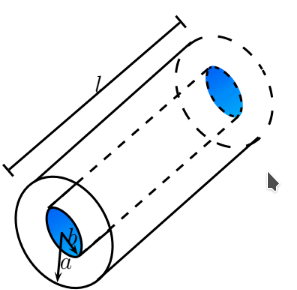
\includegraphics[scale=0.6]{resistencia-fuga}
\end{minipage}




\item Existe una clase de metales y compuestos cuya resistencia virtualmente desaparece al llegar a cierta temperatura crítica $T_{c}$. Dichos materiales son conocidos como \textbf{Superconductores}. Estudie dicho fenómeno.


\item Estime el costo de prender una bombilla de $100$ $W$ durante $12$ $h$. Suponga que dicha bombilla opera con una diferencia de potencial $\Delta V =120$ $V$  y que el kilovatio por hora en Medellín es de $1$ $KW h \approx 48.91$ pesos.

\item Costo de preparar la comida\\
Estime el costo de cocinar un pavo durante $4$ h en un horno que opera de manera continua a $20.0$ A y a $240$ V de la siguiente forma:
\begin{enumerate}
\item Calcule la potencia.
\item Calcule la energía gastada.
\item Investigue en su cuenta de servicios públicos cuanto vale el KWh (kilovatio-hora) y calcule el costo. 
\end{enumerate}

\item Cuatro resistencias se conectan como se muestra en la figura.

\begin{minipage}{11 cm}{
\begin{enumerate}
\item Encuentre la resistencia equivalente entre los puntos $a$ y $c$.
\item Cul es la corriente en cada resistencia si una diferencia de potencial de $42$ V se mantiene entre los puntos $a$ y $c$?
\end{enumerate}
}\end{minipage}
\begin{minipage}{5 cm}{
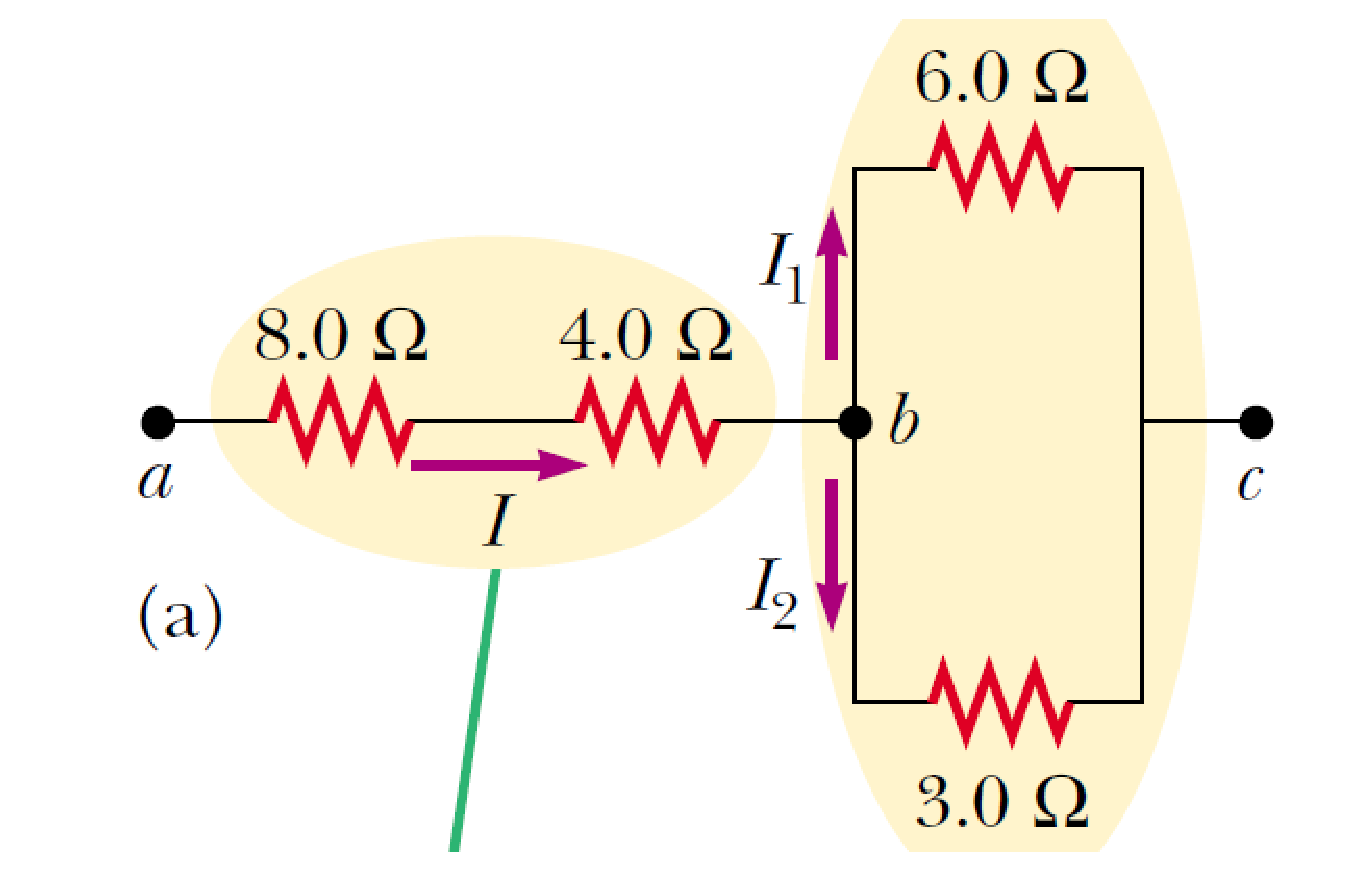
\includegraphics[scale=0.3]{grafica-resistencia}
}\end{minipage}

\item Tres resistencias son conectadas en paralelo. Una diferencia de potencial de $18.0$ V es establecida entre los puntos $a$ y $b$:

\begin{minipage}{11 cm}{
\begin{enumerate}
\item Halle la corriente en cada resistencia.
\item Calcule la potencia que cae en cada resistencia. 
\item Halle la potencia total.
\end{enumerate} 
}
\end{minipage}
\begin{minipage}{5 cm}{
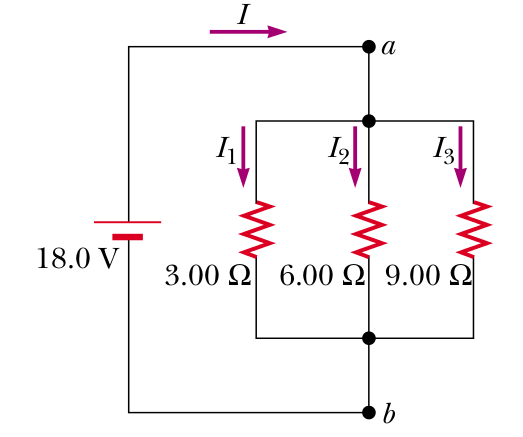
\includegraphics[scale=0.3]{grafica-3resistencias}
}\end{minipage}

\begin{minipage}{11 cm}{
\item Halle la resistencia equivalente entre los puntos $a$ y $b$ para el siguiente circuito (respuesta: $R_{ab}=(27/17)\Omega$).}
\end{minipage}
\begin{minipage}{5 cm}{
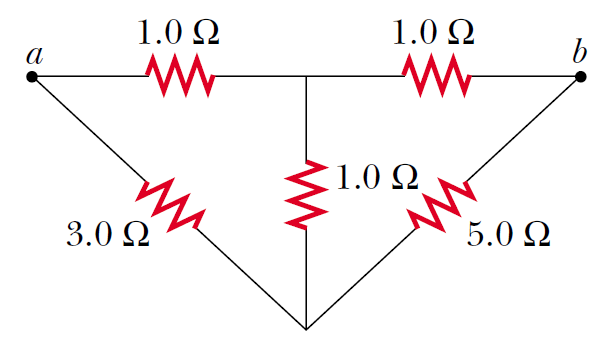
\includegraphics[scale=0.3]{grafica7}
}\end{minipage}

\vspace{1.0 cm}
LEYES DE KIRCHHOFF 

\begin{minipage}{11 cm}{
\item A single loop circuit contains two resistor and two batteries (see the graph). Find the current in the circuit (neglect the internal resistances of the batteries).}
\end{minipage}
\begin{minipage}{5 cm}{
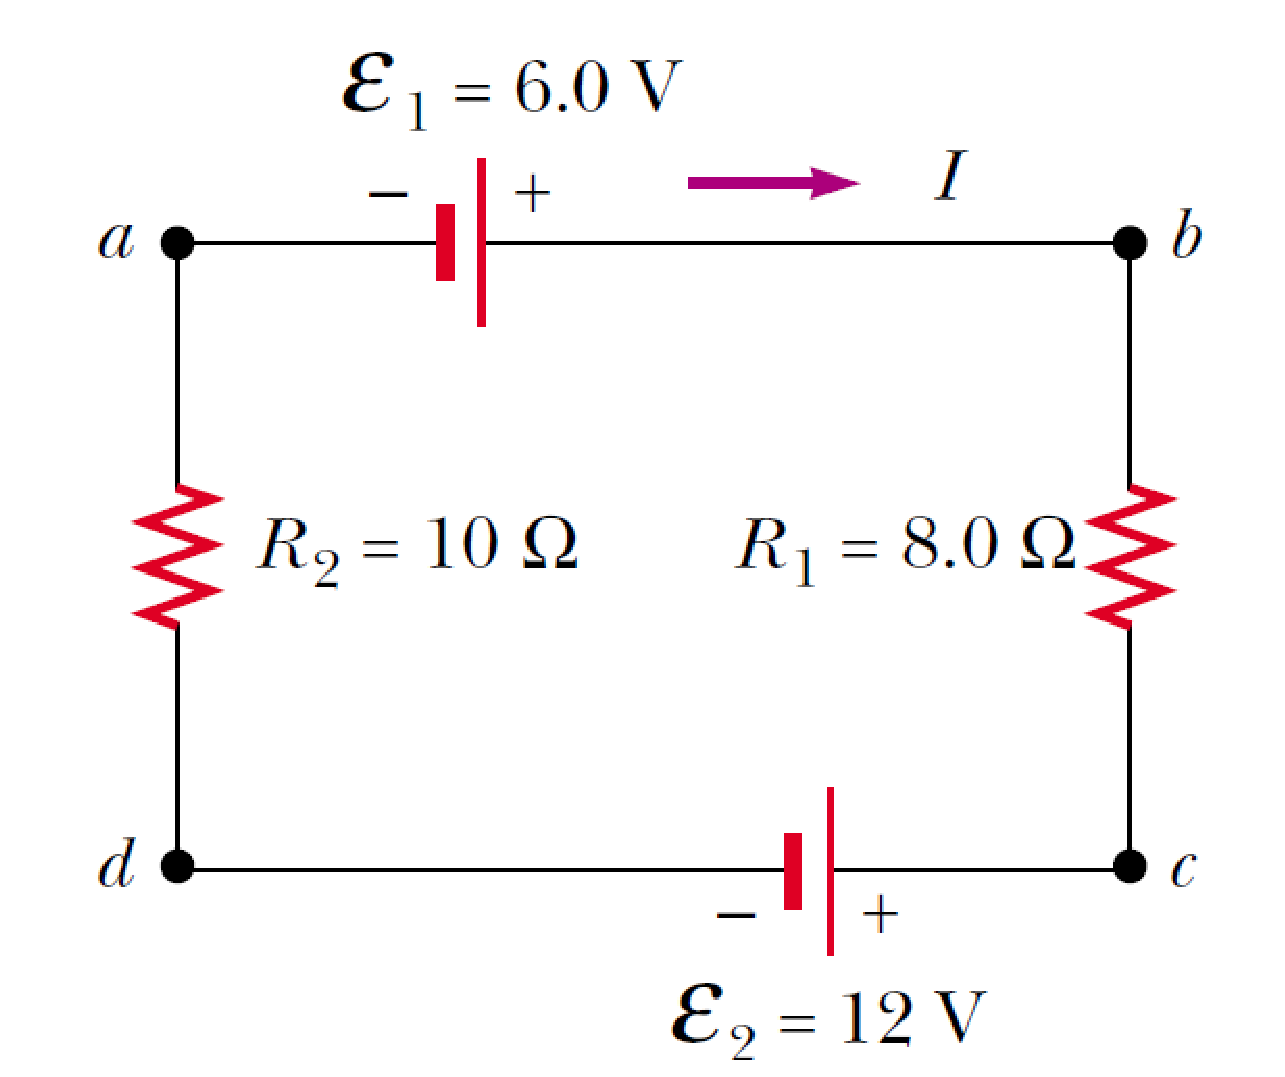
\includegraphics[scale=0.25]{grafica4}
}
\end{minipage}

\begin{minipage}{11 cm}{
\item Encuentre el valor de las corrientes en cada resistencia.}
\end{minipage}
\begin{minipage}{5 cm}{
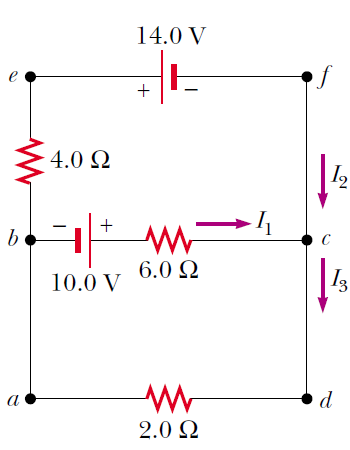
\includegraphics[scale=0.3]{grafica5}
}
\end{minipage} 


\vspace{1.0 cm}
CIRCUITOS RC\\

\begin{minipage}{11 cm}{
\item Suponga que se tiene un capacitor inicialmente descargado. Una vez se cierra el circuito se establece una corriente llenando de cargas las placas del capacitor. El capacitor incrementa su carga hasta una carga máxima tal que el campo eléctrico establecido en el capacitor hace que se llegue al equilibrio, donde la corriente es $I=0$.}
\end{minipage}
\begin{minipage}{5 cm}{
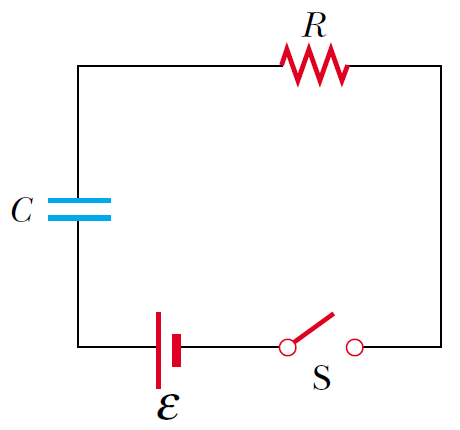
\includegraphics[scale=0.3]{grafica6}
}
\end{minipage}  

Demuestre que la corriente en el circuito y la carga en el capacitor (la cual va aumentando) están dadas por:
\begin{displaymath}
I(t)=\dfrac{\xi}{R}\exp^{-\dfrac{t}{RC}} \hspace{2 cm}
q(t)=\xi C[1-\exp^{-\dfrac{t}{RC}}]
\end{displaymath}

\item Demuestre que la mitad de la energía suministrada por la batería aparece como energía interna en el resistor y la otra mitad en el capacitor.

\item Considere un capacitor de capacitancia $C$ que está siendo descargado a través de un resistor $R$.
\begin{enumerate}
\item Despus de cunto tiempo la carga en el capacitor es un cuarto de su valor inicial mximo (expresarlo en términos de $RC$).
\item La energía almacenada en el capacitor decrece con el tiempo cuando el capacitor se está descargando. Después de cuanto tiempo la energía se reduce a un cuarto de valor inicial (expresarlo en términos de $RC$).
\end{enumerate}


\end{enumerate}
\end{document}
